%
% 3-nebenbedingungen.tex
%
% (c) 2023 Prof Dr Andreas Müller
%
\section{Nebenbedingungen
\label{buch:fuvar:section:nebenbedingungen}}
\kopfrechts{Nebenbedingungen}
Die Nullstellen des Gradienten sind Kandidaten für die Lösung
des Extremalproblems einer Funktion $f\colon\mathbb{R}^n\to\mathbb{R}$.
Oft trifft man jedoch Situation, in denen sich das Argument
$x\in\mathbb{R}^n$ der Funktion $f(x)$ nur auf einer Teilmenge
bewegen darf.
In diesem Abschnitt soll ein Verfahren beschrieben werden, wie sich
ein solches Problem exakt formulieren und lösen lässt.

%
% Nebenbedingungen
%
\subsection{Nebenbedingungen}
Wir betrachten das folgende Problem als Beispiel, wie sich 
Nebenbedingungen formulieren lassen.

%
% Ein Extremalproblem auf einer Kugeloberfläche
%
\subsubsection{Ein Extremalproblem auf einer Kugeloberfläche}
Auf der Oberfläche der Einheitskugel mit Mittelpunkt im Nullpunkt
des $(x_1,x_2,x_3)$-Koor\-di\-na\-ten\-sys\-tems sind die Extrema
der Funktion 
\begin{equation}
f(x)
=
x_2^2
-
x_1x_2
-
x_1x_3
-
x_2x_3
\label{buch:fuvar:nebenbedingungen:eqn:beispielf}
\end{equation}
zu finden.

%
% Lösung durch Umparametrisierung
%
\subsubsection{Lösung durch Umparametrisierung}
Eine erster Lösungsansatz ist, die Kugeloberfläche mit Kugelkoordinaten
\[
\begin{pmatrix}
x_1\\
x_2\\
x_3
\end{pmatrix}
=
\begin{pmatrix}
\sin\vartheta\cos\varphi\\
\sin\vartheta\sin\varphi\\
\cos\vartheta
\end{pmatrix}
\]
zu parametrisieren.
Durch Einsetzen der Parametrisierung in
\eqref{buch:fuvar:nebenbedingungen:eqn:beispielf}
entsteht die Funktion
\begin{align*}
f(\varphi,\vartheta)
&=
\sin^2\vartheta
\sin\varphi
(\sin\varphi
-
\cos\varphi)
-
(
\cos\varphi
+
\sin\varphi
)
\sin\vartheta
\cos\vartheta.
\end{align*}
Das Problem ist damit zu einem Extremalproblem in zwei Dimensionen
geworden und kann mit den bereits behandelten Methoden gelöst werden.

%
% Zusätzliche Bedingungen
%
\subsubsection{Zusätzliche Bedingungen}
Der Lösungsansatz durch Umparametrisierung wird weiter erschwert,
wenn zusätzliche Bedingungen erfüllt werden muss.
Wird zusätzlich Verlangt, dass der Punkt $x\in\mathbb{R}^3$ auf
dem Ellipsoid mit der Gleichung
\begin{equation}
g(x)
=
\begin{pmatrix}
x_1\\x_2\\x_3
\end{pmatrix}^t
\begin{pmatrix}
2&1&1\\
1&3&1\\
1&1&4
\end{pmatrix}
\begin{pmatrix}
x_1\\x_2\\x_3
\end{pmatrix}
=
1.
\label{buch:fuvar:nebenbedingungen:eqn:beispielg},
\end{equation}
liegt, dann werden die zulässigen Punkte durch eine Kurve in der
$(\varphi,\vartheta)$-Ebene beschrieben, für die eine Parametrisierung
gefunden werden muss.
Eine solche Lösung ist offenbar sehr kompliziert.
Gesucht wird ein Lösungsansatz, der ohne Umparametrisierung das folgende
allgemeine Problem löst.

\begin{aufgabe}
\label{buch:fuvar:nebenbedingungen:aufgabe:grund}
Gegeben sind stetig differenzierbare Funktionen
$f\colon\mathbb{R}^n\to\mathbb{R}$ und
$g_i\colon\mathbb{R}^n\to\mathbb{R}$ für $i=1,\dots,k$.
Man finde ein Extremum der Funktion $f(x)$ unter der Bedingungen,
dass
\[
g_1(x) = 0,\quad g_2(x)=0,\quad\dots,\quad g_k(x)=0
\]
gilt.
\end{aufgabe}

%
% Extremalaufgaben mit einer Nebenbedingung
%
\subsection{Extremalaufgaben mit einer Nebenbedingung}
In diesem Abschnitt untersuchen wir das Extremum einer stetig
differenzierbaren Funktion $f\colon\mathbb{R}^n\to\mathbb{R}$
unter der Bedinung $g(x)=0$ mit einer stetig differenzierbaren
Funktion $g\colon\mathbb{R}^n\to\mathbb{R}$.
Sei also $x_0\in\mathbb{R}^n$ so, dass $f(x_0)$ minimal ist unter
allen Punkten $x\in \mathbb{R}^n$, die die Nebenbedingungen $g(x)=0$
erfüllen.
Da $x_0$ ein Minimum ist, müssen die Werte $f(x)$ für Punkte $x$
in der Nähe von $x_0$ grösser sein, allerdings nur, wenn $x$ auch
die Bedingungen $g(x)=0$ erfüllt.

Für ein Extremalproblem ohne Nebenbedingung wurde das Verschwinden
aller Richtungsableitung als notwendige Bedingung für das
Extremum gefunden.
Tatsächlich nimmt die Funktion auch in jeder Richtung ausgehend
von $x_0$ zu.
Unter der Nebenbedingung gilt dies nicht mehr.
Nur noch Änderungen von $x$, die auch die Nebenbedingung
erfüllen, durfen in Betracht gezogen werden.
Die von $x_0$ ausgehdenden Geraden $t\mapsto x_0+vt$ mit dem
Richtungsvektor $v$ erfüllen die Nebenbedingungen nur dann, wenn
die Menge $M=\{x\in\mathbb{R}^n \mid g(x)=0\}$ Geraden enthält, also
typischerweise gar nicht.

Es müssen also Kurven $t\mapsto x(t)\in\mathbb{R}^n$ mit $x(0)=x_0$
betrachtet werden, die $g(x(t))=0$ für alle $t$ in einer kleinen Umgebung
von $0$ erfüllen.
Für ein Minimum ist dann notwendig, dass die Ableitung
\begin{equation}
0
=
\frac{d}{dt} f(x(t))\bigg|_{t=0}
=
Df(x_0)\cdot \frac{dx(t)}{dt}\bigg|_{t=0}
=
Df(x_0)\cdot \dot{x}(0)
\label{buch:fuvar:nebenbedingungen:eqn:gradf}
\end{equation}
ist.
Nicht jeder Vektor $v=\dot{x}$ kann vorkommen, da $\dot{x}(0)$ ein
Tangentialvektor der Menge $M$ ist.
Da $g(x(t))=0$ ist, sind diese Vektoren durch
\begin{equation}
0
=
\frac{d}{dt}g(x(t))\bigg|_{t=0}
=
Dg(x_0)\cdot \dot{x}(0)
=
\grad g(x_0)\cdot \dot{x}(0)
\label{buch:fuvar:nebenbedingungen:eqn:gradg}
\end{equation}
charakterisiert.
Nur Vektoren $\dot{x}(0)$, die auf dem Gradienten $\grad g(x_0)$ 
senkrecht stehen, sind zulässig.
Wir halten dieses Resultat im folgenden Lemma fest.

\begin{lemma}
\label{buch:fuvar:nebenbedingungen:lemma:nebenbedingungen}
Ist $x_0$ ein Extremum der Funktion $f(x)$ unter der Nebenbedingung
$g(x)=0$, dann verschwindet die Richtungsableitung
\(
D_vf(x_0) = \grad f(x_0)\cdot v = 0
\)
von $f$ an der Stelle $x_0$ in jeder Richtung $v$, die tangential
an die Menge $\{x\in\mathbb{R}^n \mid g(x)=0\}$ ist, für die also
$\grad g(x_0)\cdot v=0$ gilt.
\end{lemma}

Damit haben wir die folgende notwendige Bedingung gefunden.

\begin{satz}[Extremalproblem mit einer Nebenbedingung]
\label{buch:fuvar:nebenbedingungen:satz:nebenbedingung}
Sei $f\colon\mathbb{R}^n\to\mathbb{R}$ eine stetig differenzierbare
Funktion, die im Punkt $x_0\in\mathbb{R}^n$ unter allen Punkten
$x\in\mathbb{R}^n$ ein Extremum annimmt unter der Nebenbedingung
$g(x)=0$ für eine stetig differenzierbare Funktion
$g\colon\mathbb{R}^n\to\mathbb{R}$ mit nicht verschwindendem Gradienten.
Dann ist $\grad{f}(x_0)$ ein Vielfaches von $\grad{g}(x_0)$.
\end{satz}

\begin{proof}
Nach
\eqref{buch:fuvar:nebenbedingungen:eqn:gradf}
und
\eqref{buch:fuvar:nebenbedingungen:eqn:gradg}
muss 
\[
\grad f(x_0)\cdot v = 0
\]
sein für alle Vektoren $v$ mit $\grad g(x_0)\cdot v= 0$.
Der Vektor $\grad f(x_0)$ steht also auf allen Vektoren senkrecht, die
auf $\grad g(x_0)$ senkrecht stehen.
Dies trifft wegen $\grad g(x_0)\ne 0$ genau dann zu, wenn $\grad f(x_0)$
ein Vielfaches von $\grad g(x_0)$ ist.
\end{proof}

Die Lösung des Extremalproblems in
Satz~\ref{buch:fuvar:nebenbedingungen:satz:nebenbedingung}
%
% nebenbedingung.tex
%
% (c) 2024 Prof Dr Andreas Müller
%
\begin{figure}
\centering
%\vspace*{2cm}
%XXX Extremalproblem in zwei Dimensionen mit einer Nebenbedingung
%\vspace*{2cm}
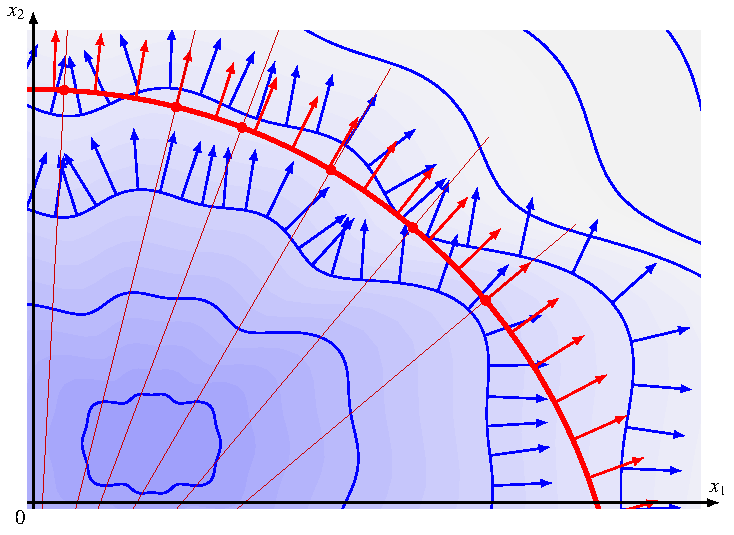
\includegraphics{chapters/010-fuvar/images/nebenbedingung.pdf}
\caption{Extremalproblem für eine Funktion ${\color{blue}f(x,y)}$
(dargestellt durch
die {\color{blue}blauen} Niveaulinien) unter einer Nebenbedingung
${\color{darkred}g(x,y)=c}$, was der Vorgabe einer Kurve
({\color{darkred}rot}), auf der das Extremum gefunden werden muss,
entspricht.
Im Extremum sind die {\color{blue}blauen} Normalen auf den Niveaulinien
$\grad f$ parallel zur {\color{darkred}roten} Normalen $\grad g$ auf
der Nebenbedingungskurve.
\label{buch:fuvar:nebenbedingung:fig:nebenbedingung}}
\end{figure}

lässt sich auch wie in
Abbildung~\ref{buch:fuvar:nebenbedingungen:fig:nebenbedingung}
visualisieren.
Die Funktion $f(x,y)$ ist durch ihre blauen Niveaulinien 
dargestellt, die Nebenbedingung durch die rote Kurve.
Das Extremum kann dort gefunden werden, wo die Normalen auf die
Niveaulinien und die rote Kurve parallel sind.
%
% lagrangekurve.tex -- slide template
%
% (c) 2021 Prof Dr Andreas Müller, OST Ostschweizer Fachhochschule
%
\bgroup
\begin{frame}[t]
\setlength{\abovedisplayskip}{5pt}
\setlength{\belowdisplayskip}{5pt}
\frametitle{Extremum mit Nebenbedingung}
\vspace*{-0.2cm}
\begin{center}
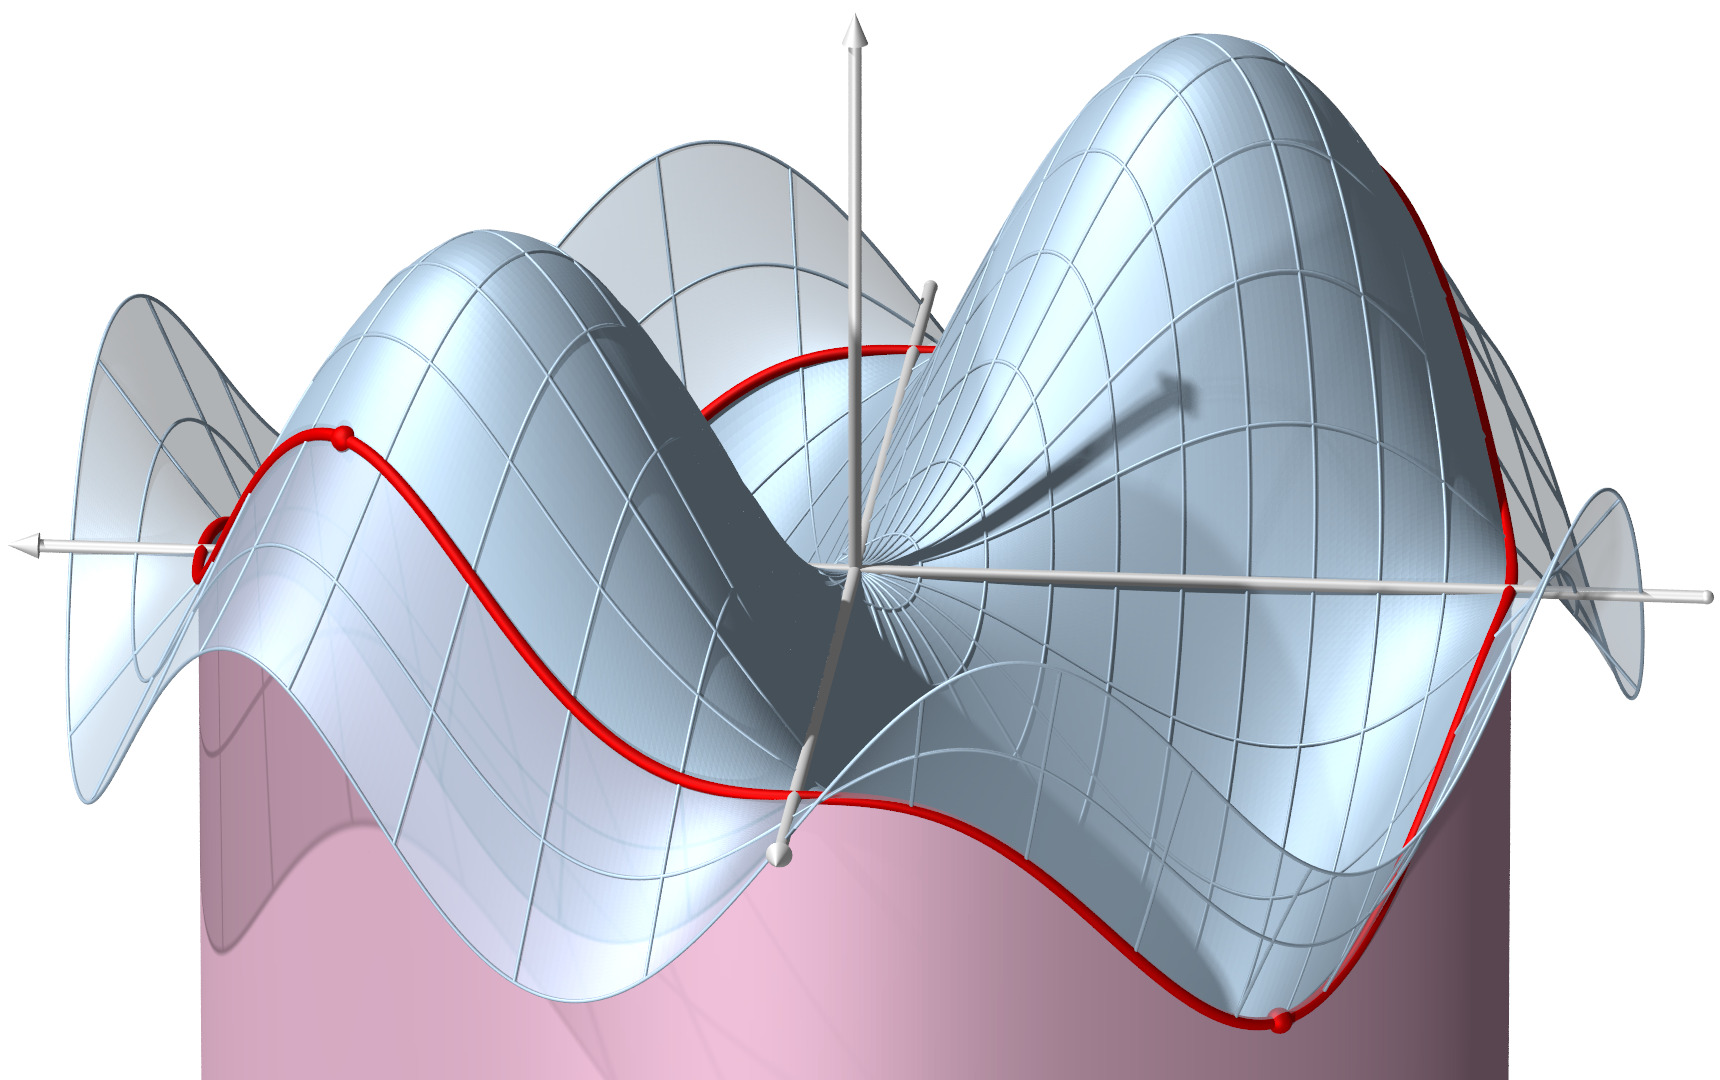
\includegraphics[width=12.3cm]{../../buch/chapters/010-fuvar/images/lagrangekurve.jpg}
\end{center}
\end{frame}
\egroup

%
% lagrangezyl.tex
%
% (c) 2021 Prof Dr Andreas Müller, OST Ostschweizer Fachhochschule
%
\documentclass[tikz]{standalone}
\usepackage{times}
\usepackage{amsmath}
\usepackage{txfonts}
\usepackage[utf8]{inputenc}
\usepackage{graphics}
\usetikzlibrary{arrows,intersections,math,calc}
\usepackage{ifthen}
\begin{document}

\newboolean{showgrid}
\setboolean{showgrid}{false}
\def\breite{7}
\def\hoehe{4}

\begin{tikzpicture}[>=latex,thick]
\clip (-6.3,-4) rectangle (6.3,4);

% Povray Bild
\node at (0,0) {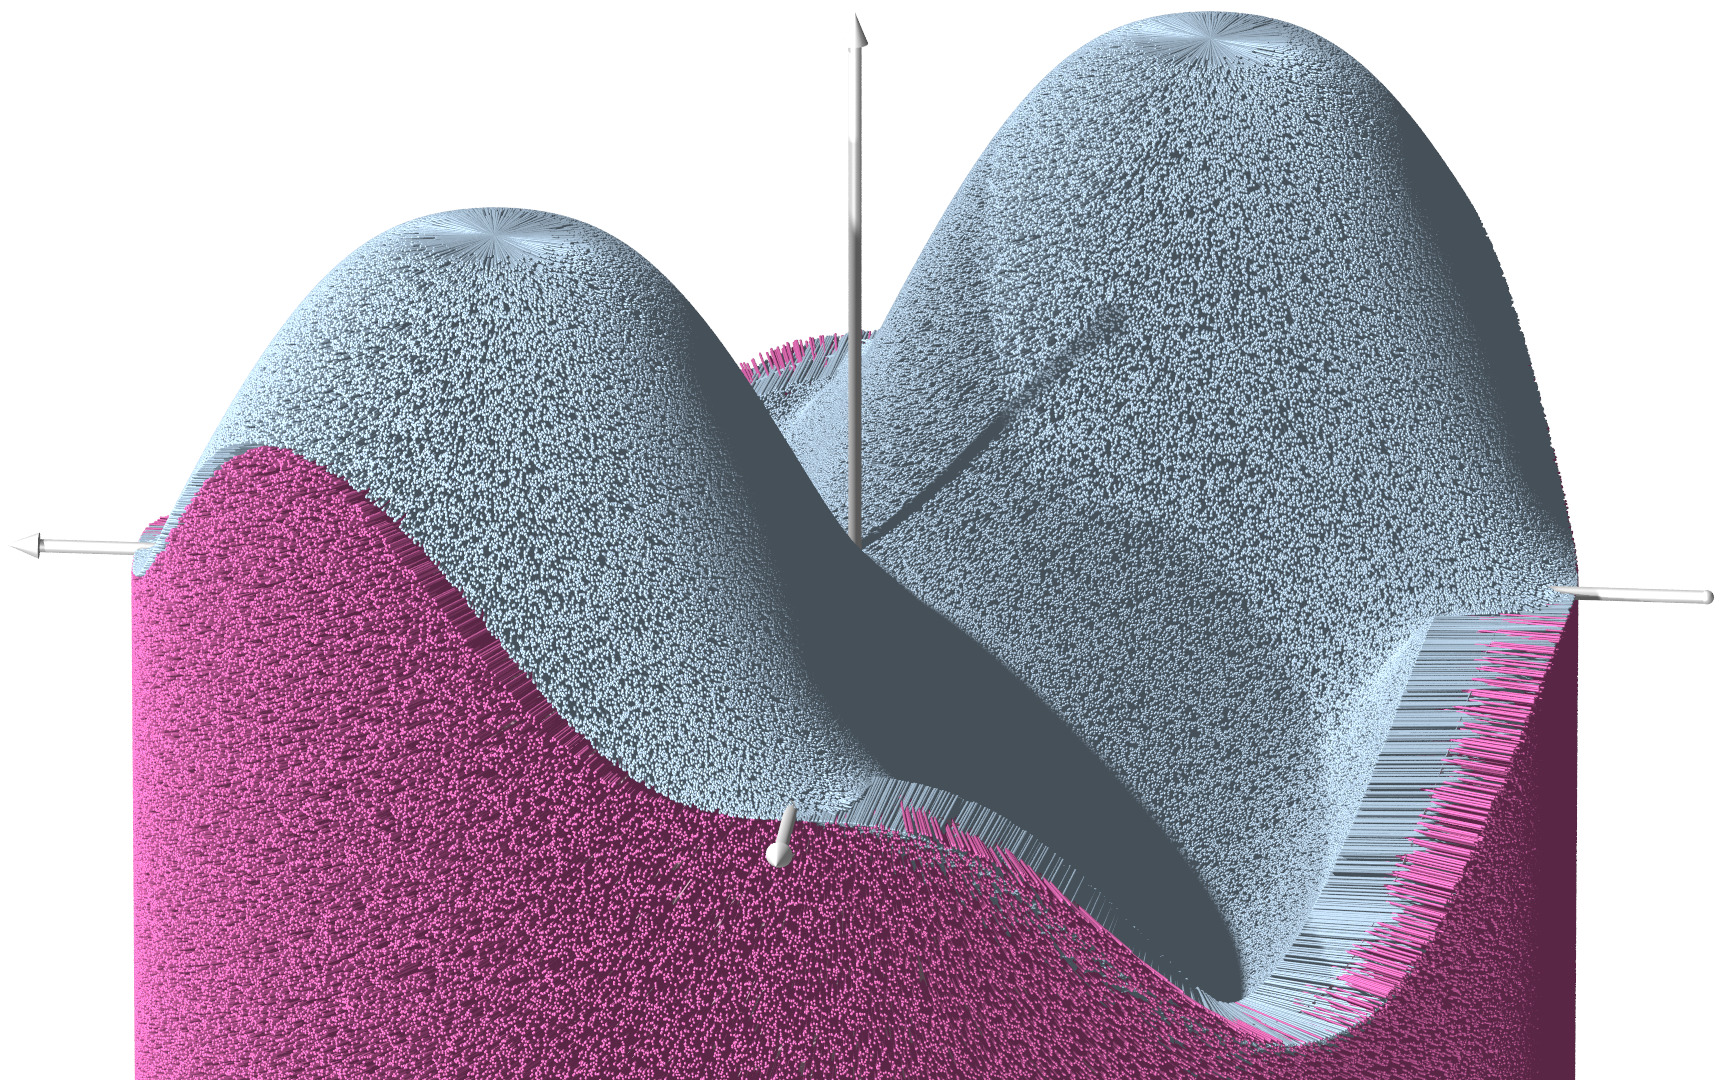
\includegraphics[width=12.6cm]{lagrangezyl.jpg}};

% Gitter
\ifthenelse{\boolean{showgrid}}{
\draw[step=0.1,line width=0.1pt] (-\breite,-\hoehe) grid (\breite, \hoehe);
\draw[step=0.5,line width=0.4pt] (-\breite,-\hoehe) grid (\breite, \hoehe);
\draw                            (-\breite,-\hoehe) grid (\breite, \hoehe);
\fill (0,0) circle[radius=0.05];
}{}


\node at (-6.1,0.2) {$x$};
\coordinate (Y) at (-0.6,-2.65);
\fill[color=white,opacity=0.5] ($(Y)+(-0.15,-0.2)$) rectangle +(0.3,0.4);
\node at (Y) {$y$};
\node at (-0.2,3.8) {$z$};

\end{tikzpicture}

\end{document}

Eine dreidimensionale Visualisierung ist zudem in den 
Abbildungen
\ref{buch:fuvar:nebenbedingungen:fig:lagrangekurve}
und
\ref{buch:fuvar:nebenbedingungen:fig:lagrangezyl}
gegeben.
In
Abbildung~\ref{buch:fuvar:nebenbedingungen:fig:lagrangezyl}
sind die Richtungen der Gradienten $\operatorname{grad} f(x,y)$ als
hellblaue und des Gradienten $\operatorname{grad}g(x,y)$ als hellrote
``Haare'' dargestellt.
Nur bei den Extrema sind die ``Haare'' parallel.

Als praktisches Beispiel sei auf
Abbildung~\ref{buch:fuvar:nebenbedingung:fig:karte}
verwiesen.
%
% karte.tex
%
% (c) 2024 Prof Dr Andreas Müller
%
\begin{figure}
\centering
\includegraphics{chapters/010-fuvar/images/karteextremum.pdf}
\caption{Lokale Maxima ({\color{darkred}rote} Kreise) und Minima
({\color{blue}blaue} Kreise) der Höhe entlang eines Wanderwegs
({\color{gelb}gelb}) sind Lösungen eines Extremalproblems.
Die Nebenbedingung ist der Wanderweg, der einschränkt, wo der Wanderer
sich bewegen kann.
Die zu optimierenden Grösse $f(x,y)$ ist die Höhe.
Extreme treten an stellen auf, wo die Höhenlinien, die Niveaulinien 
von $f$ und der Wanderweg parallel verlaufen.
\label{buch:fuvar:nebenbedingung:fig:karte}}
\end{figure}

Der {\color{gelb}gelbe} Wanderweg schränkt den Wanderer ein,
er ist einen Nebenbedingung für die Bewegung des Wanderers.
Die Höhe $f(x,y)$ als Funktion der $x$-$y$-Koordinaten wird in
der Karte durch die Höhenlinien dargestellt.
Der Wanderer kommt genau dann bei einem lokalen Maximum oder
Minimum vorbei, wenn Wanderweg und Höhenlinien parallel sind.

\begin{beispiel}
Wir lösen die eingangs gestellte Aufgabe, die Extrema der Funktion
$f(x)$ von \eqref{buch:fuvar:nebenbedingungen:eqn:beispielf}
unter der Nebenbedingung zu finden, dass $|x|=1$ ist.
Die Funktion $g(x)$ ist
\[
g(x)
=
x_1^2 + x_2^2 + x_3^2 - 1.
\]
Die Gradienten von $f$ und $g$ sind
\[
\grad f(x)
=
\begin{pmatrix*}[r]
-x_2-x_3\\
-x_1+2x_2-x_3\\
-x_1-\phantom{2}x_2\phantom{\mathstrut-x_3}
\end{pmatrix*}
\qquad\text{und}\qquad
\grad g(x)
=
\begin{pmatrix}
2x_1\\
2x_2\\
2x_3
\end{pmatrix}
=
2x.
\]
Kandidaten für Extremale sind Punkte, in denen die beiden Gradienten
proportional sind, für die also das Gleichungssystem
\begin{equation}
\left.
\begin{aligned}
\grad f({\color{darkred}x})&=\lambda \grad g({\color{darkred}x})\\
      g({\color{darkred}x})&=0
\end{aligned}
\quad
\right\}
\qquad\Rightarrow\qquad
\left\{
\quad
\renewcommand\arraycolsep{2pt}
\begin{array}{rcrcrcr}
	&-& {\color{darkred}x_2}
		&-& {\color{darkred}x_3}
			&=& 2{\color{darkred}\lambda x_1}\\
-{\color{darkred}x_1}
	&+& 2{\color{darkred}x_2}
		&-& {\color{darkred}x_3}
			&=& 2{\color{darkred}\lambda x_2}\\
-{\color{darkred}x_1}
	&-& {\color{darkred}x_2}
		& &
			&=& 2{\color{darkred}\lambda x_3}\\
{\color{darkred}x}^2_{\color{darkred}1}
	&+& {\color{darkred}x}^2_{\color{darkred}2}
		&+& {\color{darkred}x}^2_{\color{darkred}3}
			&=& 1
\end{array}
\right.
\label{buch:fuvar:nebenbedingungen:eqn:glsystem}
\end{equation}
Dies ist ein System von vier nichtlinearen Gleichungen für die vier
Unbekannten ${\color{darkred}x_1}$, ${\color{darkred}x_2}$,
${\color{darkred}x_3}$ und ${\color{darkred}\lambda}$.
In Matrixform lassen sich die ersten drei Gleichungen als
\begin{equation}
\underbrace{
\begin{pmatrix*}[r]
 0&-1&-1\\
-1& 2&-1\\
-1&-1& 0
\end{pmatrix*}
}_{\displaystyle = A}
{\color{darkred}x}
=
A
{\color{darkred}x}
=
2{\color{darkred}\lambda x}
\label{buch:fuvar:nebenbedingungen:eqn:evgl}
\end{equation}
schreiben.
Da die vierte Gleichung von~\eqref{buch:fuvar:nebenbedingungen:eqn:glsystem}
verlangt, dass $\color{darkred}x$ nicht der Nullvektor ist, besagt
\eqref{buch:fuvar:nebenbedingungen:eqn:evgl}, dass ${\color{darkred}}$
ein Eigenvektor von $A$ mit Eigenwert $2{\color{darkred}\lambda}$ sein muss.
Das charakteristische Polynom
\[
\det(A-tI)
=
-t^3+2t^2+3t-4
=
-(t-1)(t^2+t-4)
\]
hat die Nullstellen $t_0=1$ und
\[
t_{\pm}
=
\frac{-1\pm\sqrt{17}}{2},
\]
was auf die zulässigen Werte
\[
{\color{darkred}\lambda}_0=-\frac12,
\quad\text{und}\quad
{\color{darkred}\lambda}_\pm = \frac{1\mp\sqrt{17}}{4}
\]
für ${\color{darkred}\lambda}$ führt.
Mit etwas Geduld oder einem Computeralgebrasystem kann man auch die
zugehörigen Eigenvektoren
\[
{\color{darkred}x}_0
=
\begin{pmatrix*}[r]
 1\\
 0\\
-1
\end{pmatrix*}
\quad\text{und}\quad
{\color{darkred}x}_\pm
=
\begin{pmatrix*}
1\\
\frac{-3\pm\sqrt{17}}{2}\\
1
\end{pmatrix*}
\]
finden.
Durch Normierung lassen sich jetzt Punkte finden, die die Nebenbedingung
erfüllen und damit Kandidaten für Extrema sind.
\end{beispiel}

%
% Lagrange-Multiplikatoren
%
\subsection{Lagrange-Multiplikatoren}
Wir kehren zum allgemeinen Problem der
Aufgaben~\ref{buch:fuvar:nebenbedingungen:aufgabe:grund}
zurück.
Sei also wieder $f\colon \mathbb{R}^n\to\mathbb{R}$
und
$g_i\colon\mathbb{R}^n\to\mathbb{R}$, $i=1,\dots,k$,
stetig differenzierbare Funktionen und $x_0$ ein Extremum
von $f$ unter allen $x\in\mathbb{R}^n$ mit $g_i(x)=0$ für $i=1,\dots,k$.
Die Richtungsableitung von $f$ an der Stelle $x_0$ muss für alle
Richtungen $v$ verschwinden, die tangential an die Menge
\[
M
=
\{
x\in\mathbb{R}^n
\mid
g_1(x)=\ldots=g_k(x)=0
\}
\]
sind.
Die zulässigen Richtungen $v$ erfüllen die Bedingung
\[
\grad g_i(x_0)\cdot v  = 0,\quad i=1,\dots,k,
\]
In Matrixform sind dies die Lösungen des homogenen Gleichungssystems
\[
{\renewcommand{\arraystretch}{1.2}
\begin{pmatrix}
\displaystyle\frac{\partial g_1}{\partial x_1}(x_0)
&\dots&
\displaystyle\frac{\partial g_1}{\partial x_n}(x_0)
\\
\vdots&\ddots&\vdots\\
\displaystyle\frac{\partial g_k}{\partial x_1}(x_0)
&\dots&
\displaystyle\frac{\partial g_k}{\partial x_n}(x_0)
\end{pmatrix}}
\begin{pmatrix}
v_1\\
\vdots\\
v_n
\end{pmatrix}
=
Dg(x_0) v
=
0.
\]

\begin{satz}[Lagrange-Multiplikatoren]
\label{buch:fuvar:nebenbedingungen:satz:lm}
Seien $f\colon\mathbb{R}^n\to\mathbb{R}$ und
$g_i\colon\mathbb{R}^n\to\mathbb{R}$, $i=1,\dots,k$, stetig
differenzierbare Funktionen.
Für ein Extremum $x_0$ von $f(x)$ unter allen $x\in\mathbb{R}^n$,
die die Nebenbedingungen $g_i(x)=0$, $i=1,\dots,k$ erfüllen, ist notwendig,
dass es reelle Zahlen $\lambda_1,\dots,\lambda_k\in\mathbb{R}$ gibt derart,
dass
\[
\grad f(x_0)
=
\lambda_1\grad g_1(x_0)
+\ldots+
\lambda_k\grad g_k(x_0)
=
\sum_{i=1}^k \lambda_i \grad g_i(x_0)
\]
gilt.
Kandidaten für Extrema von $f$ unter den Nebenbedingungen $g_i(x)=0$ sind
daher Lösungen des Gleichungssystems
\begin{equation}
\begin{aligned}
\grad f({\color{darkred}x})
&=
\sum_{i=1}^k {\color{darkred}\lambda_i} g_i({\color{darkred}x})
\\
g_i({\color{darkred}x})
&= 
0\qquad i=1,\dots k
\end{aligned}
\label{buch:fuvar:nebenbedingungen:eqn:lm}
\end{equation}
für ${\color{darkred}x}$ und ${\color{darkred}\lambda_i}$, $i=1,\dots,k$.
\end{satz}

Die erste Gleichung des Gleichungssytems
\eqref{buch:fuvar:nebenbedingungen:eqn:lm}
ist eine $n$-dimensionale Vektorgleichung, entspricht also $n$
Komponentengleichungen.
Sie kann auch geschrieben werden als ein lineares Gleichungssystem
mit $n$ Gleichungen für die Variablen
${\color{darkred}\lambda_1},\dots,{\color{darkred}\lambda_k}$
mit der Koeffizientenmatrix $Dg(x_0)^t$.
Die Nebenbedingungen steuern $k$ weitere Gleichungen bei.
Insgesamt ist \eqref{buch:fuvar:nebenbedingungen:eqn:lm}
daher ein im Allgemeinen nichtlineares Gleichungssystem von $n+k$
Gleichungen für die $n+k$ Unbekannten
\(
{\color{darkred}x_1},\dots,{\color{darkred}x_n},
{\color{darkred}\lambda_1},\dots,{\color{darkred}\lambda_k}
\).
Leider kann man keine allgemeinen Lösungsverfahren für solche
Gleichungen erwarten.
Eine interessante Ausnahme liegt vor, wenn die Funktionen $f$ und $g_i$
quadratische Funktionen sind, dies wird im
Abschnitt~\ref{buch:fuvar:section:quadratisch}
untersucht.

Alternativ kann man den Satz
\ref{buch:fuvar:nebenbedingungen:satz:lm}
auch so formulieren:

\begin{satz}
\label{buch:fuvar:nebenbedingungen:satz:lm2}
Unter den Voraussetzungen von Satz~\eqref{buch:fuvar:nebenbedingungen:satz:lm}
ist für ein Extremum von $f$ unter den Nebenbedingungen $g_i$, $i=1,\dots,k$,
notwendig, dass
es relle Zahlen $\lambda_1,\dots,\lambda_k\in\mathbb{R}$ derart gibt,
dass 
\[
\grad\biggl(f-\sum_{i=1}^k \lambda_ig_i\biggr)(x_0) = 0
\qquad\text{und}\qquad
g_i(x_0)=0\quad \forall i=1,\dots,k
\]
gilt.
\end{satz}

